%%%%%%%% ICML 2023 EXAMPLE LATEX SUBMISSION FILE %%%%%%%%%%%%%%%%%

\documentclass[nohyperref]{article}

% Recommended, but optional, packages for figures and better typesetting:
\usepackage{microtype}
\usepackage{graphicx}
\usepackage{subfigure}
\usepackage{booktabs} % for professional tables

% hyperref makes hyperlinks in the resulting PDF.
% If your build breaks (sometimes temporarily if a hyperlink spans a page)
% please comment out the following usepackage line and replace
% \usepackage{icml2023} with \usepackage[nohyperref]{icml2023} above.
\usepackage{hyperref}


% Attempt to make hyperref and algorithmic work together better:
\newcommand{\theHalgorithm}{\arabic{algorithm}}

% Use the following line for the initial blind version submitted for review:
\usepackage[accepted]{icml2023}

% If accepted, instead use the following line for the camera-ready submission:
% \usepackage[accepted]{icml2022}

% For theorems and such
\usepackage{amsmath}
\usepackage{amssymb}
\usepackage{mathtools}
\usepackage{amsthm}

% if you use cleveref..
\usepackage[capitalize,noabbrev]{cleveref}

%%%%%%%%%%%%%%%%%%%%%%%%%%%%%%%%
% THEOREMS
%%%%%%%%%%%%%%%%%%%%%%%%%%%%%%%%
\theoremstyle{plain}
\newtheorem{theorem}{Theorem}[section]
\newtheorem{proposition}[theorem]{Proposition}
\newtheorem{lemma}[theorem]{Lemma}
\newtheorem{corollary}[theorem]{Corollary}
\theoremstyle{definition}
\newtheorem{definition}[theorem]{Definition}
\newtheorem{assumption}[theorem]{Assumption}
\theoremstyle{remark}
\newtheorem{remark}[theorem]{Remark}

% Todonotes is useful during development; simply uncomment the next line
%    and comment out the line below the next line to turn off comments
%\usepackage[disable,textsize=tiny]{todonotes}
\usepackage[textsize=tiny]{todonotes}


% The \icmltitle you define below is probably too long as a header.
% Therefore, a short form for the running title is supplied here:
\icmltitlerunning{Sample RL Project Proposal}

\newcommand{\dnl}{\mbox{}\par}
\newcommand{\mycomment}[1]{\textbf{Note:} \textit{#1}}
\newcommand{\cnote}[1]{\textsf{\color{blue} [#1]}}
%\newcommand{\cnote}[1]{}


\begin{document}

\twocolumn[
\icmltitle{RL Project Checkpoint}

% It is OKAY to include author information, even for blind
% submissions: the style file will automatically remove it for you
% unless you've provided the [accepted] option to the icml2022
% package.

% List of affiliations: The first argument should be a (short)
% identifier you will use later to specify author affiliations
% Academic affiliations should list Department, University, City, Region, Country
% Industry affiliations should list Company, City, Region, Country

% You can specify symbols, otherwise they are numbered in order.
% Ideally, you should not use this facility. Affiliations will be numbered
% in order of appearance and this is the preferred way.
\icmlsetsymbol{equal}{*}

\begin{icmlauthorlist}
\icmlauthor{Airi Shimamura}{} %{equal,yyy}
\icmlauthor{Khoi Trinh}{} %{equal,yyy,comp}
%\icmlauthor{Firstname3 Lastname3}{comp}
%\icmlauthor{Firstname4 Lastname4}{sch}
%\icmlauthor{Firstname5 Lastname5}{yyy}
%\icmlauthor{Firstname6 Lastname6}{sch,yyy,comp}
%\icmlauthor{Firstname7 Lastname7}{comp}
%\icmlauthor{}{sch}
%\icmlauthor{Firstname8 Lastname8}{sch}
%\icmlauthor{Firstname8 Lastname8}{yyy,comp}
%\icmlauthor{}{sch}
%\icmlauthor{}{sch}
\end{icmlauthorlist}

%\icmlaffiliation{yyy}{Department of XXX, University of YYY, Location, Country}
%\icmlaffiliation{comp}{Company Name, Location, Country}
%\icmlaffiliation{sch}{School of ZZZ, Institute of WWW, Location, Country}

%\icmlcorrespondingauthor{Amy McGovern}{first1.last1@xxx.edu}
%\icmlcorrespondingauthor{Anna Partner}{first2.last2@www.uk}

% You may provide any keywords that you
% find helpful for describing your paper; these are used to populate
% the "keywords" metadata in the PDF but will not be shown in the document
%\icmlkeywords{Machine Learning, ICML}

\vskip 0.3in
]

% this must go after the closing bracket ] following \twocolumn[ ...

% This command actually creates the footnote in the first column
% listing the affiliations and the copyright notice.
% The command takes one argument, which is text to display at the start of the footnote.
% The \icmlEqualContribution command is standard text for equal contribution.
% Remove it (just {}) if you do not need this facility.

%\printAffiliationsAndNotice{}  % leave blank if no need to mention equal contribution
%\printAffiliationsAndNotice{\icmlEqualContribution} % otherwise use the standard text.

For our RL project this semester; we want to build an RL agent that can easily beat the CartPole game.  

CartPole v1 is a game environment provided in the Gym package from OpenAI. In this environment, there is a pole, attached to a cart (hence the name CartPole). The cart moves along a frictionless track. Force is applied in the left and right direction of the cart.
The goal of the game is to keep the pole upright for as long as possible. For each step taken, a +1 reward is given, including the termination step. The maximum points achievable in the game is 475. There are a few conditions that, if met, will end the game.

In this checkpoint document, we will provide details and update on our current experiments. A slight change from the proposal, Airi are implmeneting Q-Learning, while Khoi will be implementing SARSA learning instead.

\subsection*{Airi}
For Airi's progress, she was able to create a code that successfully play the game using a Q-learning algorithm.

\subsection*{Khoi}
For Khoi's progress, he is in the process of implmeneting a SARSA training algorithm. 
The SARSA algorithm is a popular reinforcement learning algorithm. At each time step, the agent selects an action according to its policy, observes the next state and reward, and updates the estimated value of the current state-action pair using a learning rate and discount factor. 
The algorithm maintains a Q-value function that estimates the expected future rewards for each state-action pair. The agent selects an action using an exploration-exploitation strategy and takes the selected action in the environment.

To this end, Khoi is trying to implement an $\epsilon$ greedy method for this SARSA algorithm. For his setup, the hyperparameters are: $\epsilon = 0.1$; $\gamma = 0.9$; and $\alpha = 0.5$

For the criteria related to the CartPole environment, the agent will play the game for 850 episodes, and in each episodes, 100 steps will have their rewards recorded, in order to generate an average.
If the failing conditions is met, a penalty of -10 is given, otherwise, a reward of +1 is given.

For one run of 850 episodes, here are his current results. Note that due to the random nature of taking actions, each run will produce a different graph.

\begin{figure}[H] %h forces the figure to be inserted right here
    \centering
    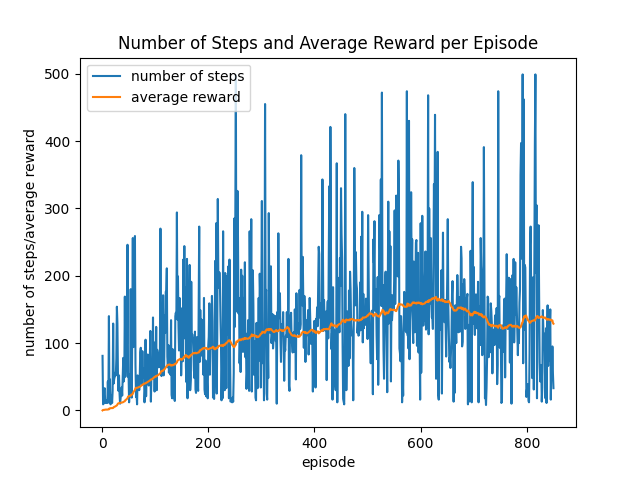
\includegraphics[width=1\linewidth]{sarsa-average.png}
    \caption{SARSA Results}
\end{figure}

\subsection*{Difficulties}

\subsection*{Future Work}
%\cnote{All written proposals must be no longer than one page per number of people in the group.}

\bibliographystyle{mslapa}
\bibliography{my,book}

\end{document}


% This document was modified from the file originally made available by
% Pat Langley and Andrea Danyluk for ICML-2K. This version was created
% by Iain Murray in 2018, and modified by Alexandre Bouchard in
% 2019 and 2021 and by Csaba Szepesvari, Gang Niu and Sivan Sabato in 2022. 
% Previous contributors include Dan Roy, Lise Getoor and Tobias
% Scheffer, which was slightly modified from the 2010 version by
% Thorsten Joachims & Johannes Fuernkranz, slightly modified from the
% 2009 version by Kiri Wagstaff and Sam Roweis's 2008 version, which is
% slightly modified from Prasad Tadepalli's 2007 version which is a
% lightly changed version of the previous year's version by Andrew
% Moore, which was in turn edited from those of Kristian Kersting and
% Codrina Lauth. Alex Smola contributed to the algorithmic style files.
